\documentclass[border=0.2cm]{standalone}
% Required packages and libraries
\usepackage{circuitikz}
\usetikzlibrary{calc}
 
\begin{document}
 
 
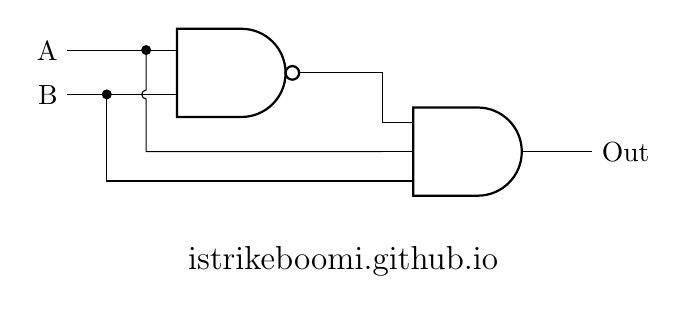
\begin{tikzpicture}
 
% Circuit style
\ctikzset{
    logic ports=ieee
}
\node[nand port] (NAND1) at (0,0) {};
\node[and port,number inputs = 3] (AND1) at (3,-1) {};
\draw (NAND1.in 1) -- ++(-1,0) node[left] (A) {A};
\draw (NAND1.in 2) -- ++(-1,0) node[left] (B) {B};
\draw (NAND1.out) -| (AND1.in 1);
\draw (AND1.in 2) -| ++(-3,.225) to[crossing] ++(0,1) to[short,-*] ++(0,.065);
\draw (AND1.in 3) -- ++(-3.5,0) to[short,-*] ++(0,1.1);
\draw (AND1.out) -- ++(.5,0) node[right] (Out) {Out};
%\node [and port] (AND1) at (0,0) {};
%\node [or port] (OR1) at (0,-2) {};
%\draw (NOT1.in) -- ++(-1,0) node[left] (A) {A};
%\draw (NOT1.out) -| (AND1.in 1);
%\draw (AND1.in 2) -- ++(-2,0) node[left] (B) {B};
%\draw (OR1.in 1) -- ++(0,.95) to[crossing] ++(0,1) to[short,-*] ++(0,.05);
%\draw (OR1.in 2) -- ++(-1,0) to[short,-*] ++(0,2);
%\draw (AND1.out) -| ++(.5,0) node[right] (Out) {Out 1};
%\draw (OR1.out) -| ++(.5,0) node[right] (Out) {Out 2};

%\node[or port] (OR1) at (0,0) {};
%\node[and port] (AND1) at (0,-2) {};
%\node[or port] (OR2) at (0,-4) {};
%\draw (OR1.in 1) -- ++(-1,0) node[left] (A) {A};
%\draw (OR1.in 2) -- ++(-1,0) node[left] (B) {B};
%\draw (AND1.in 1) -- ++(-.25,0) to[short,-*] ++(0,1.45);
%\draw (AND1.in 2) -- ++(-1,0) node[left] (C) {C};
%\node[not port,rotate=270,scale=.5] (NOT1) at (-1.5,-3.2825) {};
%\draw (NOT1.in) -- ++(0,.075) to[crossing] ++(0,1) to[short,-*] ++(0,2.05);
%\draw (NOT1.out) -| (OR2.in 1);
%\draw (OR2.in 2) -| ++(-.75,0) to[short,-*] ++(0,2);
%
%\node[xor port, number inputs = 3] (XOR1) at (3,-2) {};
%\draw (OR1.out) -| (XOR1.in 1) node[above] {};
%\draw (AND1.out) -| (XOR1.in 2) node[above] {};
%\draw (OR2.out) -| (XOR1.in 3) node[above] {};
%\draw (XOR1.out) -- ++(.5,0) node[right] (Out) {Out};
%\node[and port] (AND1) at (0,0) {};
%\node[nor port] (NOR1) at (0,-2) {};
%\draw (AND1.in 1) -- ++(-1,0) node[left] (A) {A};
%\draw (AND1.in 2) -- ++(-1,0) node[left] (B) {B};
%\draw (NOR1.in 1) -- ++(-1,0) node[left] (C) {C};
%\draw (NOR1.in 2) -- ++(-1,0) node[left] (D) {D};
%
%\node[xor port] (XOR1) at (3,-1) {};
%\draw (AND1.out) -| (XOR1.in 1) node[above] {};
%\draw (XOR1.in 2) -| ++(-3,0) to[short, -*] ++(0,1) node[left] {};
%
%\node [xnor port] (XNOR1) at (6,-1) {};
%\draw (NOR1.out) -| (XNOR1.in 2) node[above] {};
%\draw (XOR1.out) -| (XNOR1.in 1);
%\draw (XNOR1.out) -- ++(.5,0) node[right] (Out) {Out};

%\node[and port] (AND1) at (0,0) {};
%\node[and port] (AND2) at (0,-2) {};
%\node[not port] (NOT1) at (2,-.7225) {};
%\node[or port] (OR1) at (4,-1) {};
%\draw (AND1.in 1) -- ++(-1,0) node[left] (A) {A};
%\draw (AND1.in 2) -| ++(-0,0) to[short,-*] ++(0,-.70) to[short] ++(-.95,0) node[left] (B) {B};
%\draw (-1.05,-1) -| (AND2.in 1) node[left] {};
%\draw (AND1.out) -| (NOT1.in) node[left] {};
%\draw (NOT1.out) -- (OR1.in 1) node[above] {};
%\draw (AND2.in 2) -- ++(-1,0) node[left] (C) {C};
%\draw (AND2.out) -| (OR1.in 2) node[left] {};
%\draw (OR1.out) node[right] (Out) {};

%\node[xor port, number inputs = 3] (XOR){};
%\draw (XOR.in 1) -- ++(-1.5,0)node[left](A){A};
%\draw (XOR.in 2) -- ++(-1.5,0)node[left](B){B};
%\draw (XOR.in 3) -- ++(-1.5,0)node[left](C){$C_{in}$};
%\draw (XOR.out) -- ++(.5,0) node[right]{Sum};
%
%% AC
%\node[and port] (AND1) at (0,-2){};
%\draw (AND1.in 1) -| ++(-0.25,2.1) coordinate(A1) node[circ] at (A1) {};
%\draw (AND1.in 2) -| ++(-0.75,1.9) coordinate(temp) node[circ] at (temp) {};
%% BC
%\node[and port] (AND2) at (0,-4){};
%\draw (AND2.in 1) -| ++(-0.5,0) to[short] ++(0,1) to[crossing] ++(0,.9) to[short,-*] ++(0,1.8);
%\draw (AND2.in 2) -| ++(-0.75,2.25) coordinate(temp) [xing] {};
%
%% AB
%\node[and port] (AND3) at (0,-6){};
%\draw (AND3.in 1) -| ++(-0.25,0) to[short] ++(0,1) to[crossing] ++(0,.9) to[crossing] ++(0,.2) to[crossing] ++(0,2.65) to[short, -*] ++(0,-.75);
%\draw (AND3.in 2) -| ++(-0.5,0) to[short] ++(0,1.55) to[crossing] ++(0,.9) to[short,-*] ++(0,.1);
%
%\node[or port, number inputs = 3] (OR) at (3,-4){};
%\draw (OR.in 1) -| (AND1.out);
%\draw (OR.in 2) -| (AND2.out);
%\draw (OR.in 3) -| (AND3.out);
%\draw (OR.out) -- ++(.5,0) node[right]{$C_{out}$};


%% Logic ports
%\node[or port] (ORa) at (0,0){};
%\node[not port] (Noa) at (0,-2){};
%\node[or port] (ORb) at (0,-4){};
% 
%\node[not port] (Nob) at (2.5,0){};
%\node[and port] (ANDa) at (2.5,-3){};
% 
%\node[or port] (ORc) at (5,-1.5){};
% 
%% Connection
%\draw (ORa.out) -- (Nob.in);
% 
%\draw (Noa.out) -| (ANDa.in 1);
%\draw (ORb.out) -| (ANDa.in 2);
% 
%\draw (ANDa.out) -|  (ORc.in 2);
%\draw (Nob.out) -| (ORc.in 1);
%\draw (ORc.out) -- ++(1,0) node[near end,above]{Out};
% 
%\draw (ORa.in 1) -- ++(-1.5,0)node[left](In1){In1};
%\draw (ORb.in 2) -- ++(-1.5,0)node[left](In3){In3};
% 
%% Jump crossing element
%\node at (ORa.in 2)
%[
%    below,
%    jump crossing,
%    rotate=-90,
%    scale=1.3
%](X){};
% 
%\draw (Noa.in) -| (X.east)
%    (X.west) to[short,-*] (X.west |- ORa.in 1); 
% 
%\draw ($ (In1) !.5! (In3) $) node[]{In2}
%    ++ (0.4,0) to[short,-*] ++(0.5,0) coordinate(a)
%    |- (X.south) (a) |- (ORb.in 1);
\node[anchor=north, yshift=-5mm, font=\large]
    at (current bounding box.south)
      {istrikeboomi.github.io};
\end{tikzpicture}
\end{document}